\chapter{Narzędzia do symulacji sieci}
% Wykorzystany symulator zdarzeń dyskretnych, opisać po krótce inne
% 1-2 strony
Rozdział ten opisuje narzędzia oraz technologie, które zostały użyte do symulacji działania sieci czujników, implementacji protokołów trasowania oraz przeprowadzenia testów.

Projekty dotyczące  bezprzewodowych sieci czujnikowych są skompliowane zarówno w swojej złożoności, jak i skali. Konieczne stało się więc umożliwienie badania bezprzewodowych sieci czujnikowych w kontrolowanych warunkach. Z powodu wysokich nakładów finansowych oraz pracy jakie wiązałyby się z przeprowadzeniem takich testów z fizycznym sprzętem do tego celu wykorzystywane są symulacje stworzone w środowisku wirtualnym. Użyteczne oprogramowanie symulacyjne powinno spełniać  następujące cechy \cite{Xian2008}:
\begin{itemize}
	\item Oprogramowanie symulacyjne powinno kłaść szczególny nacisk na rozbudowane narzędzia do analizy modeli symulacyjnych.
	
	\item Struktura modeli powinna odzwierciedlać hierarchiczną strukturę bezprzewodowych sieci czujnikowych. Modele powinny składać się z powiązanych ze sobą komponentów, które można ponownie wykorzystywać, co umożliwia przyśpieszenie prac nad symulacjami.
	
	\item Oprogramowanie symulacyjne powinno definiować otwarty interfejs dla danych, aby możliwe było przetwarzanie danych wejściowych oraz wyjściowych za pomocą zewnętrznych narzędzi (np. możliwość załadowania danych wynikowych do bazy danych, wykorzystanie danych wynikowych w celu stworzenia wykresów oraz raportów).
\end{itemize}
\section{Narzędzia komercyjne}
\paragraph{QualNet \cite{Kellner10simulationenvironments}}
Komercyjny symulator sieci stworzony przez firmę Scalable Technologies. Umożliwia tworzenie modeli sieci składających się z trasowników, przełączników, serwerów, punktów dostępowych, radioodbiorników, anten wraz z gotowymi protokołami trasowania. Dodatkowo QualNet zawiera graficzny interfejs użytkownika wraz z narzędziem do projektowania scenariuszy symulacyjnych, wizualizatorami 2D i 3D oraz analizatorem pakietów i statystyk.

\paragraph{OPNET \cite{Fahmy2016}}
OPNET (Optimized Network Engineering Tool) powstał w 1987 roku, jako pierwszy komercyjne narzędzie do symulacji sieci komunikacyjnych. Zawiera w sobie rozbudowane środowisko programistyczne umożliwiające ich specyfikację, symulację oraz analizę wydajnościową. Wspierany jest przy tym szeroki zakres tych sieci, począwszy od prostych sieci LAN, a skończywszy na globalnych sieciach satelitarnych. OPNET jest symulatorem zdarzeń dyskretnych umożliwiającym analizę wydajnościową oraz zachowanie symulowanych systemów. Wspieranymi językami programowania są C oraz Java. Narzędzie to jest wykorzystywane w szerokim zakresie do badania działania protokołu TCP w standardzie ATM. Dodatkowo zawiera on implementacje takich protokołów trasowania jak: OSPF, RIP, EIGRP, BGP, IGRP, DSR, TORA, PNNI oraz gotowe implementacje MAC, mobilności węzłów, modeli poboru energii czy modeli należących do warstwy aplikacji.
Oprócz wersji komercyjnej istnieje również darmowa wersja akademicka oprogramowania, jednakże zawiera ona tylko wcześniej zaimplementowane przez twórców modele protokołów oraz urządzeń bez możliwości dodania własnych lub modyfikacji istniejących. Jej głównym przeznaczeniem są symulacje różnych topologii sieci.
\begin{figure}[H]
	\begin{center}
		\centering
		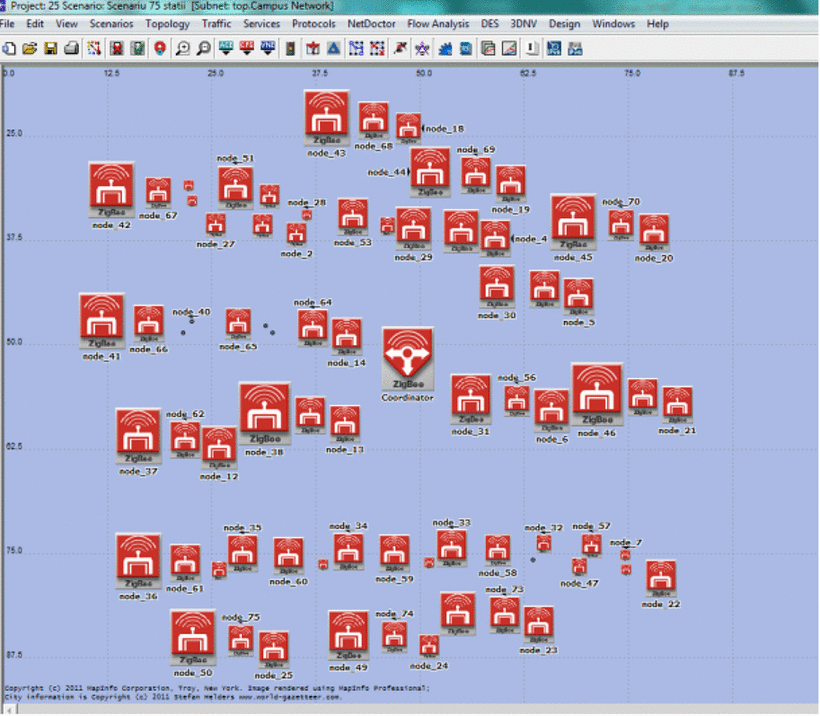
\includegraphics[scale=0.5]{\ImgPath/tools/opnet.png} 
	\end{center}
	\caption{OPNET - przykładowy widok zawierający scenariusz z 75 węzłami. Źródło: \cite{MarghescuC.2011Soaw}}
	\label{opnet}
\end{figure}
\paragraph{Matlab/Simulink}
MATLAB/Simulink jest oprogramowaniem przeznaczonym do obliczeń numerycznych wyprodukowanym przez firmę Mathworks Inc.  Część pakietu o nazwie Simulink umożliwia modelowanie, symulację oraz analizę dynamicznych systemów. Dodatkowo zawiera on wiele narzędzi (toolkits) związanych z takimi domenami jak: przetwarzanie sygnałów cyfrowych, systemy sterowania, komunikacja czy systemy wbudowane. Dzięki dostępnym narzędziom możliwe jest stworzenie modeli symulacyjnych zintegrowanych z modelami sprzętowymi. Jest to popularne rozwiązanie w dziedzinie bezprzewodowych sieci czujnikowych. Matlab/Simulink jest dostępny na platformach Windows, Mac OS X i Linux \cite{Rajaram2016}. 
\section{Narzędzia otwarte}
\paragraph{NS-2} Jest to uznany symulator zdarzeń dyskretnych stworzony w 1989 roku. W symulatorze wykorzystywane są dwa języki: C++ oraz OTcl (Object Oriented Tool Command Language). C++ używany jest do implementacji protokołów oraz rozszerzania biblioteki symulacyjnej. Z kolei w języku OTcl pisane są skrypty, których zadaniem jest konfiguracja symulacji, topologii sieci, tworzenie scenariuszy testowych i prezentacja wyników \cite{Heidemann2018, Meeneghan2004}. Do jego zalet z punktu widzenia symulacji bezprzewodowych sieci czujnikowych należą gotowe implementacje protokołów takich jak np. 802.11, 802.16, 802.15.4. Niestety nie zapewnia on symulacji  procesów badanych przez czujniki oraz wykorzystywany przez niego model zużycia energii, formaty pakietów i protokoły MAC odbiegają znacznie od tych używanych w rzeczywistych implementacjach bezprzewodowych sieci czujnikowych. Brak jest również wsparcia dla warstwy aplikacji. NS-2 dostępny jest za darmo.
\paragraph{NS-3 \cite{Nsnam}}
Podobnie jak NS-2, NS-3 jest również uznanym symulatorem zdarzeń dyskretnych. Nie stanowi on jednak rozszerzenia ani kontynuacji NS-3. Jest to kompletnie nowy symulator z całkowicie innym interfejsem programistycznym. W NS-3 wszystkie symulacje pisane są w czystym C++, z możliwością skorzystania z Pythona. Nie posiada on interfejsu graficznego - w celu graficznej prezentacji wyników konieczne jest skorzystanie z zewnętrznych narzędzi. Zawiera moduły implementujące 802.15.4, 6LoWPAN i RPL.
\paragraph{TOSSIM \cite{Musznicki2012}}
TOSSIM jest emulatorem bezprzewodowych sieci czujnikowych opartym na systemie operacyjnym TinyOS. 
\paragraph{J-Sim \cite{Sobeih2006}}
Jest to symulator oparty o architekturę komponentową. Umożliwia korzystanie z różnych języków skryptowych, takich jak Perl, Tcl i Python. J-Sim zawiera bibliotekę dedykowaną do symulacji bezprzewodowych sieci czujnikowych. Umożliwia przeprowadzanie symulacji z liczbą węzłów przekraczającą 1000.
\begin{figure}[H]
	\begin{center}
		\centering
		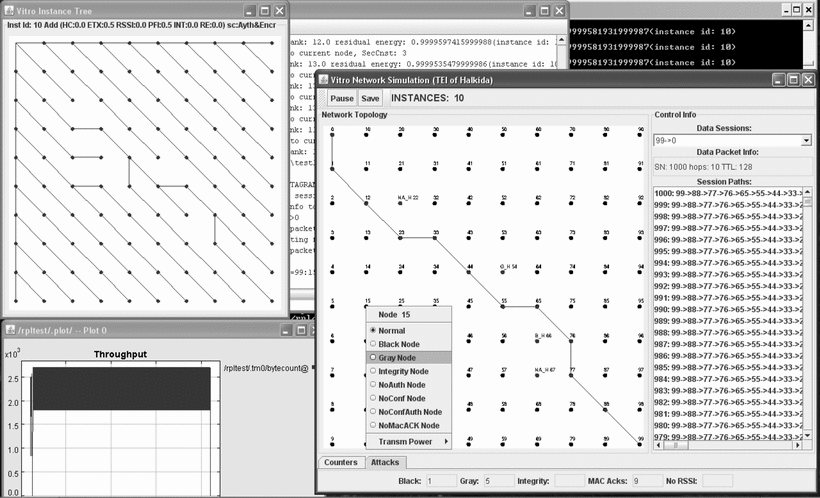
\includegraphics[scale=0.6]{\ImgPath/tools/jsim.png} 
	\end{center}
	\caption{Przykładowa symulacja w J-Sim. Źródło: \cite{KarkazisP.2012RmiJ}}
	\label{jsim}
\end{figure}
\section{\omnetpp}
\omnetpp jest zbudowanym w sposób modularny symulatorem zdarzeń dyskretnych. Stanowi on ogólne narzędzie umożliwiające przeprowadzanie symulacji między innymi: przewodowych oraz bezprzewodowych sieci komputerowych, systemów wieloprocesorowych, chmur obliczeniowych czy też ruchu miejskiego. Dla każdej bardziej wyspecjalizowanej dziedziny konieczne jest stworzenie nowego modelu (zbioru modułów) lub skorzystanie z jednego z już istniejących rozwiązań (np. INET, VEINS).\cite{Varga2017}
\subsection{Moduły}
Podstawowym budulcem symulacji w \omnetpp są moduły. Dzielą się one na proste oraz złożone.
% Opis co to moduł oraz że są proste i złożone, możne je zagneżdżać oraz wiązać za pomocą bram (ang. gate). A komunikują się za pomocą wiadomości i sygnałów

Do implementacji modułów wykorzystuje się dwa języki
\begin{enumerate}
	\item NED - język domenowy \omnetpp, za pomocą którego definiowane są moduły. Zawierają opis parametrów oraz bram modułu. Dodatkowo w przypadku modułów złożonych definiowane są zagnieżdżone moduły wraz z ich połączeniami.
	%Wstawić przykład
	\item C++ - wykorzystywany do implementacji modułów prostych (moduły złożone definiowane są tylko za pomocą plików NED).
	%Wstawić przykład
\end{enumerate}
Dodatkowo, w celu przyspieszenia oraz ułatwienia implementacji wiadomości, które moduły wykorzystują w komunikacji stworzono odpowiedni język dziedzinowy, który tłumaczony jest przez kompilator do kodu C++.
%Wstawić przykład

Moduły umieszczane są w Sieciach (Network), które również zdefiniowane są w języku NED.

Do komunikacji moduły wykorzystują zdefiniowane (w pliku .ned) przez programistę łącza (ang. links ) oraz bramy (ang. gates).
\subsection{Przeprowadzenie symulacji}
\omnetpp umożliwia skorzystanie z różnych interfejsów użytkownika: QT, TKenv oraz wiersza poleceń. W fazie testowania poprawności przygotowanej symulacji skorzystać można z jednego z interfejsów graficznych. Po weryfikacji zalecana jest rezygnacja z interfejsu graficznego w celu przyspieszenia działania symulacji. Niebywałym ułatwieniem w przygotowaniu oraz uruchomieniu zestawu symulacji w celu zebrania danych do analizy są pliki konfiguracyjne. Umożliwiają one określenie parametrów modułów wchodzących w skład sieci oraz zadeklarowanie parametrów wchodzących w skład zmiennych badanych w ramach symulacji (parameter studies).
%Wstawić przykład
\section{INET}
INET jest biblioteką/modelem zawierającym implementacji wielu protokołów sieciowych (m.in. IPv4, IPv6, TCP, SCTP, UDP), jak również standardów komunikacji wykorzystywanych m.in. w sieciach czujników (IEEE 802.15.4)\cite{inet}. Biblioteka ta stanowi rozszerzenie dla platformy \omnetpp, tak więc wykorzystuje ona tą samą koncepcję dotyczącą komunikacji pomiędzy modułami za pomocą przekazywanych wiadomości. Protokoły sieciowe reprezentowane są za pomocą modułów prostych, których interfejs zewnętrzny opisywany jest w pliku NED, a implementacja w klasie języka C++. Moduły proste wykorzystywane są w modułach z złożonych za pomocą których definiowane są urządzenia sieciowe (np. trasownik). Oprócz protokołów wykorzystywane są one również do implementacji tabel tras, mobilności węzłów oraz automatycznych konfiguratorów sieci. Modele interfejsów sieciowych takich, jak np. Ethernet, czy 802.11 również tworzone są jako moduły złożone.

Warta wspomnienia jest również alternatywa do pakietu INET (w zakresie symulacji bezprzewodowych sieci czujnikowych) jaką jest symulator Castalia. Jest to otwarte, niekomercyjne rozwiązanie oparte na oprogramowaniu \omnetpp. W przeciwieństwie do \omnetpp i INET nie jest ono jednak aktywnie rozwijane. 
